\begin{figure*}[h!]
\centering
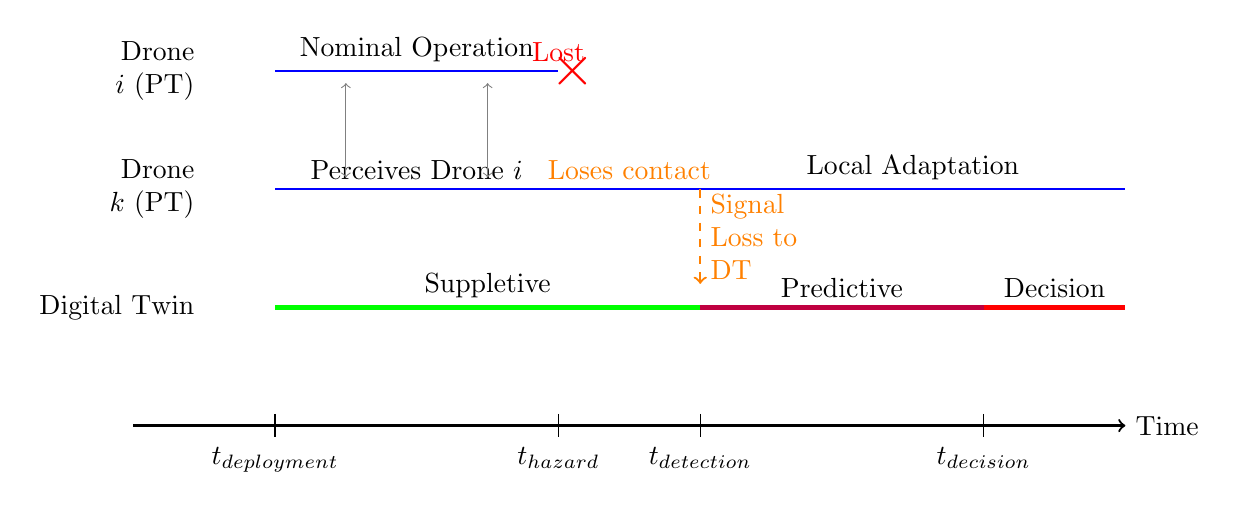
\begin{tikzpicture}[x=1.8cm, y=1.5cm]
    % Time axis
    \draw[->, thick] (0,0) -- (7,0) node[right] {Time};

    % Time markers
    \node[below] at (1,-0.1) {$t_{\text{deployment}}$};
    \draw (1,0.1) -- (1,-0.1);
    \node[below] at (3,-0.1) {$t_{\text{hazard}}$};
    \draw (3,0.1) -- (3,-0.1);
    \node[below, text width=1.5cm, align=center] at (4,-0.1) {$t_{\text{detection}}$};
    \draw (4,0.1) -- (4,-0.1);
    \node[below, text width=2cm, align=center] at (6,-0.1) {$t_{\text{decision}}$};
    \draw (6,0.1) -- (6,-0.1);

    % Drone i track (Lost)
    \node[left, text width=2cm, align=right] at (0.5, 3) {Drone $i$ (PT)};
    \draw[blue, thick] (1,3) -- (3,3);
    \node[above] at (2,3) {Nominal Operation};
    \node[red, xshift=5pt] at (3,3) {\huge $\times$};
    \node[above, red] at (3,3) {Lost};

    % Drone k track (Detects loss)
    \node[left, text width=2cm, align=right] at (0.5, 2) {Drone $k$ (PT)};
    \draw[blue, thick] (1,2) -- (7,2);
    \node[above] at (2,2) {Perceives Drone $i$};
    \draw[<->, gray] (1.5, 2.9) -- (1.5, 2.1);
    \draw[<->, gray] (2.5, 2.9) -- (2.5, 2.1);
    \node[above, orange] at (3.5,2) {Loses contact};
    \draw[->, orange, thick, dashed] (4, 2) -- (4, 1.2) node[midway, right, text width=1.5cm] {Signal Loss to DT};
    \node[above] at (5.5, 2) {Local Adaptation};

    % Digital Twin High-Level Phases
    \node[left, text width=2cm, align=right] at (0.5, 1) {Digital Twin};
    \draw[green, ultra thick] (1,1) -- (4,1);
    \node[above] at (2.5, 1) {Suppletive};
    \draw[purple, ultra thick] (4,1) -- (6,1);
    \node[above] at (5, 1) {Predictive};
    \draw[red, ultra thick] (6,1) -- (7,1);
    \node[above] at (6.5, 1) {Decision};

\end{tikzpicture}
\caption{High-level temporal sequence of PT/DT interaction. A hazard triggers detection by a PT drone, which sends an exception report to the DT. The DT transitions from a low-emission \emph{suppletive} state to an active \emph{predictive} state to analyze the situation, and then enters a \emph{decision} phase (e.g., spare injection, alert/strike recommendation).}
\label{fig:timeline_high_level}
\end{figure*}

